\section{Modeling}

\begin{definition}[\textit{System}]
    A system denoted by $\mathcal{S}$ refers to a physical entity designed to convert inputs into outputs.
\end{definition}
\begin{definition}[\textit{Model}]
    A model, symbolized as $\mathcal{M}$, constitutes a mathematical description of a system.
\end{definition}

\begin{figure}[H]
    \centering
    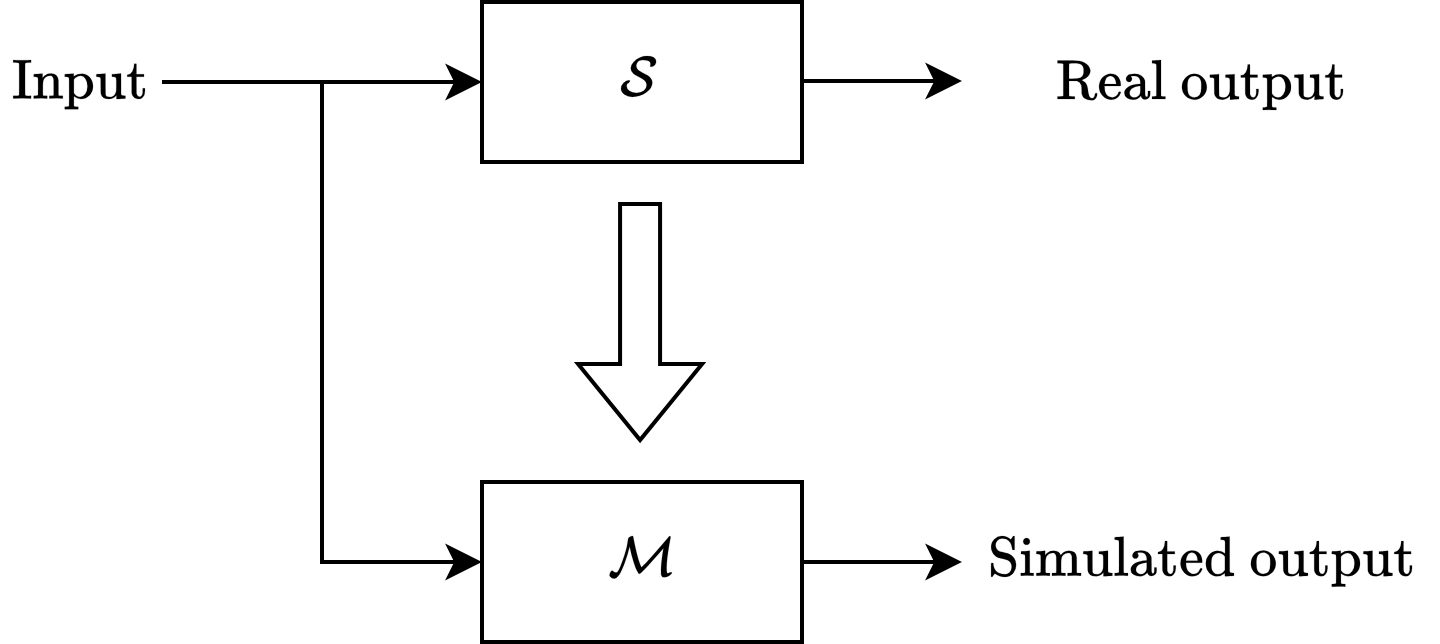
\includegraphics[width=0.5\linewidth]{images/model.png}
    \caption{Visual representation of system and model}
\end{figure}

A model can be constructed through various methodologies:
\begin{enumerate}
    \item \textit{White-box modeling}: this approach relies on established physical laws or existing knowledge. 
        The resultant model is typically generalizable, with clear physical interpretations for each variable.
        However, precise knowledge of all parameters beforehand is necessary, making it a costly and time-intensive process. 
        Consequently, it's often impractical for complex systems.
    \item \textit{Black-box modeling}: this method is based on experimental data. 
        Parameters of the model are estimated using statistical relationships derived from the data. 
        It's feasible even without in-depth knowledge of the underlying processes, and it's comparatively faster and less expensive. 
        However, models generated through this method lack physical interpretability and may not be universally applicable; changes in the system often necessitate repeating the experiment.
    \item \textit{Gray-box modeling}: hybrid methodology that commences with equations where only certain parameters are unknown. 
        Its goal is to ascertain these parameters by leveraging both statistical correlations and physical principles. 
        The benefits include the clear interpretation of variable significance and faster model construction compared to white-box approaches. 
        However, a prerequisite for gray-box modeling is the possession of some prior knowledge.
\end{enumerate}